\label{Software architecture views}
\section{Software architecture views}
This chapter discusses the architecture of the system. First we will go over the subsystem decomposition of the architecture. Then we will discuss the relation between hardware and software in the second paragraph. The third paragraph explains the data management. And the fourth paragraph describes the concurrency of the system.

\subsection{Subsystem decomposition}

The component diagram at \textbf{figure~\ref{fig:comp_diag}} shows the relations between the Tygron API, the connector and the GOAL agent. 

\begin{figure}[h]
	  \centering
	  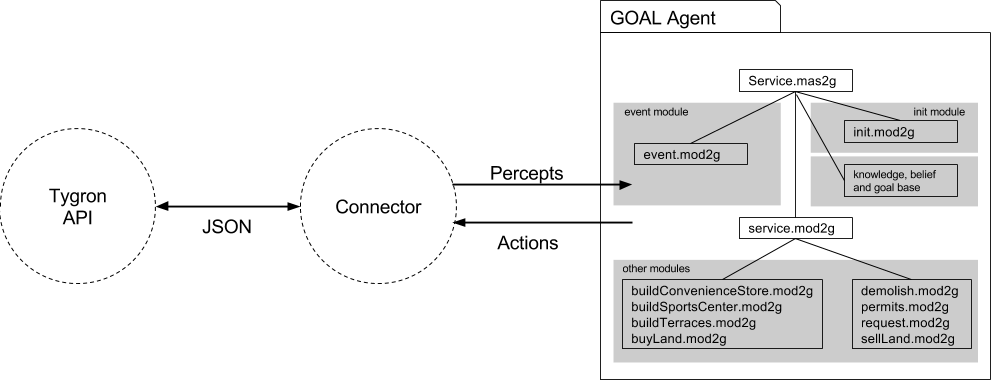
\includegraphics[width=0.7\textwidth]{system_decomposition}
	  \caption{The component diagram}
	  \label{fig:comp_diag}
\end{figure}
This figure shows the different components the project uses and how they connect to each each other. You can see how our bot connects to the connector which in turn will connect to the Tygron API. The Tygron API is extended by the module SDK (software development kit) which consists of all the graphics and calculations, basicly the Tygron game itself. The Connector uses the environment module, which is everything needed to connect an agent to the game and get and send information from the virtual human to the game. Finally, the GOAL agent consists of all the modules needed to run the bot.

\subsubsection{Connector}
The connector is extended by a contextproject package of which all Virtual Human project teams are contributers. This extended environment provides the virtual human with a lot more possible functionality through more percepts and custom built actions. The package contains both functional code and test code. The importance of having this extension is the ability of performing bigger computations on data, which would be nigh impossible in GOAL.

\subsubsection{GOAL agent}
Our GOAL Multi Agent System is started from the \texttt{service.mas2g} file, which is more or less the main class from which everything happens. This file tells the environment to connect to a session and launches the service agent. The knowledge, belief and goal base are instantiated and subsequently the \texttt{init.mod2g} is launched. This init module insert all data it needs at the start of the game into the belief base of the virtual human. After the initialisation, the event module(\texttt{event.mod2g}) and the main module(\texttt{service.mod2g}) are run alternately. In the event module every incoming percept for that cycle is handled. The main module decides what actions the agent will take by following the programmed rules and using the goals, beliefs and knowledge as data. The correct module will be called wherein even more rules have to be met. Our virtual human consits of eight extending modules, each providing a specific functionnality of the virtual human. There are three build modules for building the specific service. A module for buying land takes into account in which zone we need land the most. The demolish module sells non beneficial buildings. For communicating with other stakeholders in the game we have two special modules dealing with requests. \texttt{permits.mod2g} is desgined to ask the municipality for building permits, whereas \texttt{request.mod2g} answers land offers for buying from and selling to other stakeholders.

\subsection{Hardware/software mapping}
Our virtual human uses a different connection approach to the server than a real human user. When a session is created via the server, a user connects through its own client to that session. \textbf{figure~\ref{fig:Hard_soft_map}} shows that our virtual human will connect to the session using the context specific connector to connect with the Tygron SDK, which in turn handles the connection to the server. Visualisation of the actions performed by the virtual human are visible through a seperate instance of the Tygron Engine.

\begin{figure}[h]
	\centering
	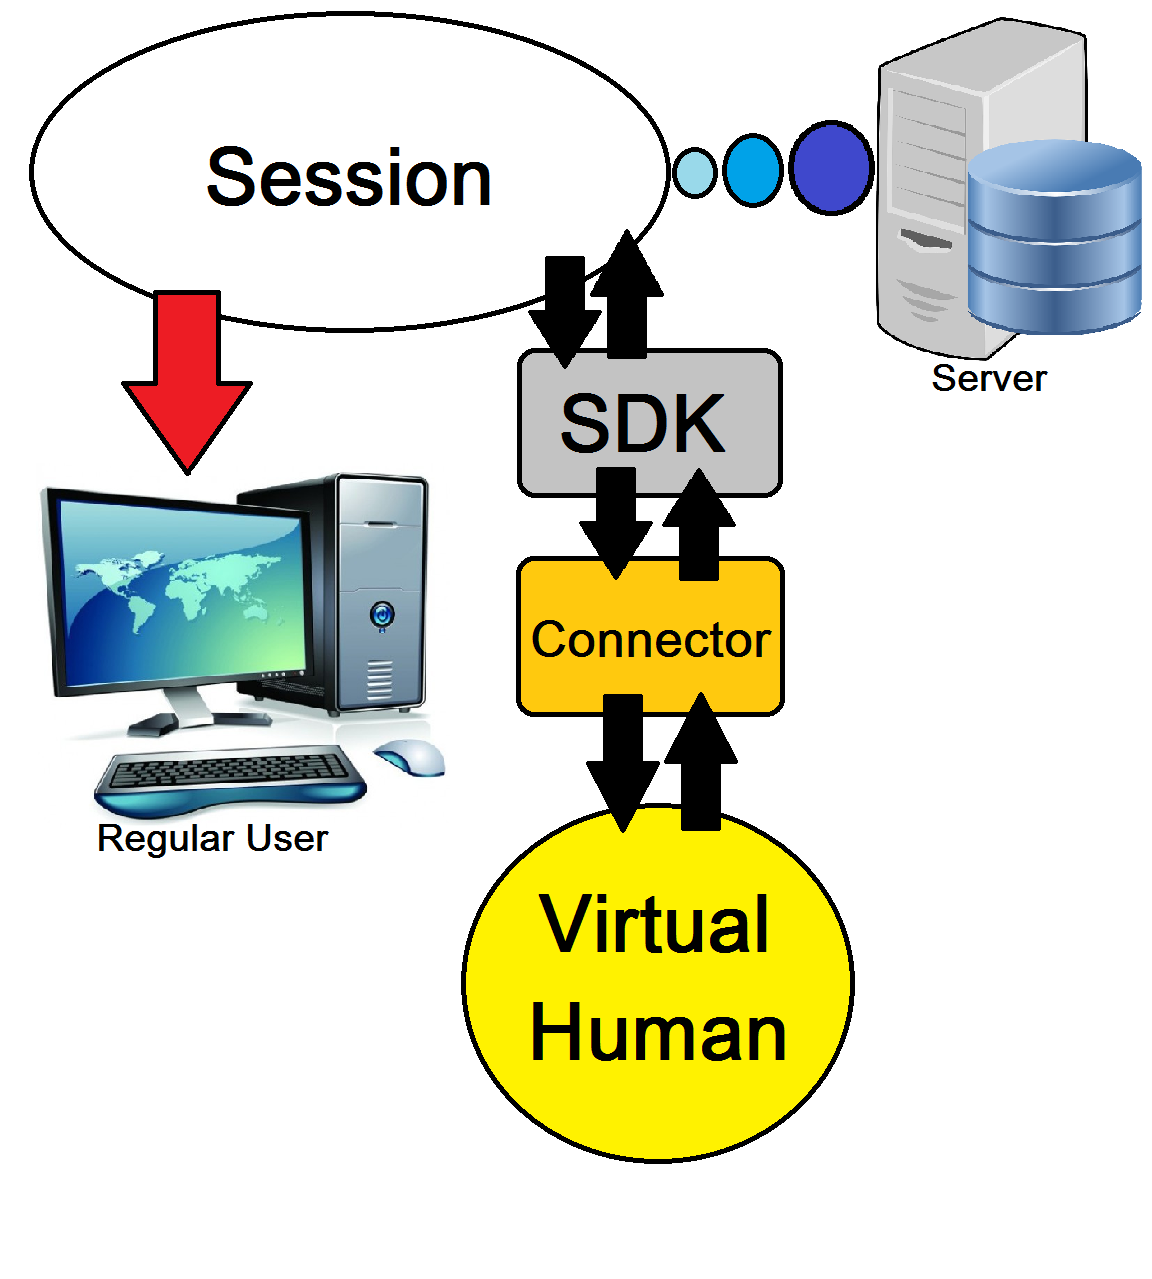
\includegraphics[width=0.5\textwidth]{Hardware_software_mapping}
	\caption{Hardware software mapping}
	\label{fig:Hard_soft_map}
\end{figure}

\subsection{Persistent data management}
When our goal connects to the Tygron engine, the engine loads the game session from its data. Everytime when our bot makes changes in the game, those changes are stored in the engine. Our bot will then read those changes from the engine and choose its next actions, which thereafter will be stored again in the engine. When our bot has reached all its goals, and there are no more updates from the game engine, the data will be kept in the Tygron engine. So our GOAL agent is not responsible for storing persistent data and it does not have external files or databases. This is so because just like a regular user would save his progress on the Tygron server, our bot will ensure everything is stored on the database of the Tygron server as well.

\subsection{Concurrency}
A GOAL agent system is designed in such a way that it always has to go through complete cycles by following the rules. Therefore, it is essential that all modules are run in the correct order. The environment also has no functionality without the input from the virtual human and is thus strongly bound to eachother; GOAL agents are interchangeble however. In practice the extending modules of the virtual human could be run out of order, but would not give the same final outcome. The fact that our GOAL agent is dependent on the Tygron engine is something unavoidable, but this causes various problems. The biggest problem is related to testing the virtual human when we need to use the Tygron engine. A Tygron server crash disrupts all sessions which then causes the Goal Agent tests to fail.

The goal agent shares resources with other users of the Tygron environment. If a deadlock occurs, this might be on the Tygron environment side and not very differently than when a deadlock would occur with human users. Deadlocks in our virtual human are prevented by covering all posible rule outcomes. Furthermore, we keep track of counters when performing certain actions. With those counters we can notice right away if something is failing and the virtual human will act accordingly to that. 
\newpage
